% introduction.tex

\newpage
\section{Introduction}
\label{chapter-introduction}
%
This report provides details on the use and validation of the Wilcox \cite{Wilcox2006}
$k$-$\omega$ turbulence model in Eilmer3. Eilmer3 is an integrated
collection of programs for the simulation of transient compressible flow
in two- and three-dimensions. Detailed descriptions of Eilmer3 can be 
found in the report by Jacobs \& Gollan \cite{Jacobs2008,Jacobs2010}, and also in reports of its
predecessor codes - CNS4U \cite{Jacobs1991}, MB\_CNS \cite{Jacobs1996}, mbcns2 \cite{Jacobs2006},
and Elmer2 \cite{Jacobs2007}. 

The implementation of the two-dimensional version of $k$-$\omega$ model in Eilmer3 has 
been done by Dr Peter Jacobs following the formulation described in the manual for
the GASPex CFD code \cite{AeroSoft2009}. Some preliminary testing on a flat plate test 
case has also been performed by J.P. Nap \cite{Nap2007}. This report extends this work 
by verifying and validating the implementation in two-dimensional flow. The extension of the 
$k$-$\omega$ model in Eilmer3 to the third dimension is currently in progress. Validation 
test cases and simulations are detailed from Chapter~\ref{chapter-flat-plate} onwards. 
Users of the code may find it convenient to identify an example close to the situation 
they wish to model and then adapt the scripts for their test case.

%------------------------------------------------------------------
\subsection{Wilcox (2006) $k$-$\omega$ model}
%\label{}
%
The Favre-averaged mass, momentum and energy conservation equations including
the equations defining the Wilcox's 2006 $k$-$\omega$ model are as follows. \\

%*** EQUATIONS EQUATIONS *****
% See Wilcox (2006) pg 255-256
Mass Conservation:
\begin{equation}
\frac{\partial \bar{\rho}}{\partial t} + \frac{\partial}{\partial x_i} 
\left( \bar{\rho} \tilde{u}_i \right) = 0
\end{equation}

Momentum Conservation:
\begin{equation}
\frac{\partial}{\partial t} \left( \bar{\rho} \tilde{u}_i \right) +
\frac{\partial}{\partial x_j} \left( \bar{\rho} \tilde{u}_j \tilde{u}_i \right) =
- \frac{\partial P}{\partial x_i} + \frac{\partial}{\partial x_j} \left[ 
\bar{t}_{ji} + \bar{\rho} \tau_{ji} \right]
\end{equation}

Energy Conservation:
\begin{eqnarray}
  \frac{\partial}{\partial t} \left[ \bar{\rho} \left( 
  \tilde{e} + \frac{\tilde{u}_i \tilde{u}_i}{2} + k \right) \right] +
  \frac{\partial}{\partial x_j} \left[ \bar{\rho} \tilde{u}_j \left( 
  \tilde{h} + \frac{\tilde{u}_i \tilde{u}_i}{2} + k \right) \right] = \nonumber \\
  \frac{\partial}{\partial x_j} \left[ 
  \left( \frac{\mu}{Pr_L} + \frac{\mu_T}{Pr_T} \right) 
  \frac{\partial \tilde{h}}{\partial x_j}  + 
  \left( \mu + \sigma^{\ast} \frac{\bar{\rho}k}{\omega} \right) 
  \frac{\partial k}{\partial x_j} \right] +
  \frac{\partial}{\partial x_j} \left[ \tilde{u}_i \left( 
  \bar{t}_{ij} + \bar{\rho}\tau_{ij} \right) \right]
\end{eqnarray}

Molecular and Reynolds-Stress Tensors:
\begin{equation}
\bar{t}_{ij} = 2 \mu \bar{S}_{ij} 
\, \, \, \, \, \, \, \, \, \, \, \, \,
\bar{\rho} \tau_{ij} = 2 \mu_T \bar{S}_{ij} - \frac{2}{3} \bar{\rho} k \delta_{ij}
\, \, \, \, \, \, \, \, \, \, \, \, \,
\bar{S}_{ij} = S_{ij} - \frac{1}{3}\frac{\partial \tilde{u}_k}{\partial x_k} \delta_{ij}
\end{equation}

Eddy Viscosity:
\begin{equation}
\mu_T = \frac{\bar{\rho} k}{\tilde{\omega}}
\, \, \, \, \, \, \, \, \, \, \, \, \,
\tilde{\omega} = \textrm{max} \left \{ \omega \, , \, \, \,
C_{lim} \sqrt{\frac{2 \bar{S}_{ij} \bar{S}_{ij}}{\beta^\ast}} \right \}
\, \, \, \, \, \, \, \, \, \, \, \, \,
C_{lim} = \frac{7}{8}
\end{equation}

Turbulence Kinetic Energy:
\begin{equation}
\frac{\partial}{\partial t} \left( \bar{\rho} k \right) +
\frac{\partial}{\partial x_j} \left( \bar{\rho} \tilde{u}_j k \right) =
\bar{\rho} \tau_{ij} \frac{\partial \tilde{u}_i}{\partial x_j} -
\beta^{\ast}\bar{\rho}k\omega + \frac{\partial}{\partial x_j} 
\left[ \left( \mu + \sigma^{\ast} \frac{\bar{\rho} k}{\omega} \right) 
\frac{\partial k}{\partial x_j}  \right]
\end{equation}

Specific Dissipation Rate:
\begin{eqnarray}
\frac{\partial}{\partial t} \left( \bar{\rho} \omega \right) +
\frac{\partial}{\partial x_j} \left( \bar{\rho} \tilde{u}_j \omega \right) =
\alpha \frac{\omega}{k} \bar{\rho} \tau_{ij} \frac{\partial \tilde{u}_i}{\partial x_j} -
\beta \bar{\rho} \omega^2 +
\sigma_d \frac{\bar{\rho}}{\omega} 
\frac{\partial k}{\partial x_j} \frac{\partial \omega}{\partial x_j} +
\frac{\partial}{\partial x_j} 
\left[ \left( \mu + \sigma \frac{\bar{\rho} k}{\omega} \right) 
\frac{\partial \omega}{\partial x_j}  \right]
\end{eqnarray}

Closure Coefficients:
\begin{equation}
\alpha = \frac{13}{25}
\, \, \, \, \, \, \, \, \, \, \, \, \,
\beta = \beta_{o} f_{\beta}
\, \, \, \, \, \, \, \, \, \, \, \, \,
\beta^{\ast} = \frac{9}{100}
\, \, \, \, \, \, \, \, \, \, \, \, \,
\sigma = \frac{1}{2}
\, \, \, \, \, \, \, \, \, \, \, \, \,
\sigma^{\ast} = \frac{3}{5}
\, \, \, \, \, \, \, \, \, \, \, \, \,
\sigma_{do} = \frac{1}{8}
\end{equation}
\begin{equation}
\beta_{o} = 0.0708
\, \, \, \, \, \, \, \, \, \, \, \, \,
Pr_T = \frac{8}{9}
\, \, \, \, \, \, \, \, \, \, \, \, \,
\sigma_{d} = \left \{
 \begin{array}{l l}
 0, & \frac{\partial k}{\partial x_j} \frac{\partial \omega}{\partial x_j} \leq 0\\
 \sigma_{do}, & \frac{\partial k}{\partial x_j} \frac{\partial \omega}{\partial x_j} > 0
 \end{array} \right .
\end{equation}
\begin{equation}
f_{\beta} = \frac{1 + 85\chi_{\omega}}{1 + 100\chi_{\omega}}
\, \, \, \, \, \, \, \, \, \, \, \, \,
\chi_{\omega} = \left | \frac{\Omega_{ij}\Omega_{jk}\hat{S}_{ki}}{\left(\beta^{\ast}\omega\right)^3} \right |
\, \, \, \, \, \, \, \, \, \, \, \, \,
\hat{S}_{ki} = S_{ki} - \frac{1}{2}\frac{\partial \tilde{u}_m}{\partial x_m} \delta_{ki}
\end{equation}
\vspace{0.5cm}

The most important differences between Wilcox's 2006 $k$-$\omega$ model
and earlier versions are the addition of a ``cross diffusion'' term and a 
built-in ``stress-limiter'' modification. The addition of ``cross diffusion'' 
(see $\sigma_d$ in the $\omega$ equation) 
was suggested as a remedy for the original $k$-$\omega$ model's sensitivity
to the freestream value of $\omega$. The ``stress-limiter'' modification
makes the eddy viscosity a function of $k$, $\omega$ and, effectively, the
ratio of turbulence-energy production to turbulence-energy dissipation.
This modification is used to improve the model's capability to predict 
hypersonic and supersonic separated flows. This modification reveals
itself as the dependence of $\mu_t$ on $\tilde{\omega}$, and is somewhat
similar to ``realisability constraints'' \cite{Moore1999}. % See Wilcox (2006) pg 280-281 
The current version also includes Pope's \cite{Pope1978} round-jet/plane-jet 
anomaly modification. This modification corrects the anomaly seen in many 
turbulence models, which wrongly predicts that a round-jet spreads more 
rapidly than a plane-jet. This modification can be seen in the 
vortex-stretching parameter $\chi_{\omega}$. The dilatation-dissipation 
modification, which improves compressible mixing layer predictions, has 
been omitted as recommended by Wilcox \cite{Wilcox2006} because it has a
detrimental effect on shock-separated flow predictions.
In addition, the boundary fudge of $\omega$ near the walls as recommended
by Menter \cite{Menter1994} has also been implemented to limit the near-wall values of
$\omega$ from becoming too large. % See Wilcox (2006) pg 386 Eq 7.17

Wilcox \cite{Wilcox1988} cites that these improvements to the $k$-$\omega$ model 
represent a significant expansion to its range of applicability. Firstly, the 
current version is as accurate as the 1988 version for attached boundary layers, 
mildly separated flows and backward-facing steps. Secondly, the current 
version's predicted free shear flow spreading rates are much closer to 
measurements than the previous version. Thirdly, the model provides 
greatly improved predictions for shock-separated flows without introducing 
any compressibility modifications to the model. Lastly, while earlier versions 
required compressibility modifications to achieve reasonable results, the 
current version has the capability to simulate flows from transonic to 
hypersonic regimes without any compressibility modifications.

%------------------------------------------------------------------
\subsection{Use of $k$-$\omega$ turbulence model in Eilmer3}
%\label{}
%
This report describes only the usage of the $k$-$\omega$ turbulence model
in Eilmer3. A more general guide to the usage of Eilmer3 can be found in
the user guide by Jacobs \& Gollan \cite{Jacobs2008}.

To activate the $k$-$\omega$ turbulence model in Eilmer3, the user
has to add the following lines to their \textit{Python} setup script.\\
\indent \texttt{gdata.viscous\_flag = 1} \\
\indent \texttt{gdata.turbulence\_flag = 1} \\
\indent \texttt{gdata.turbulence\_model = "k\_omega"} \\

In addition to these changes, the \texttt{FlowCondition()} will now
have to include two extra variables - the turbulence kinetic energy
$k$ and the specific dissipation rate $\omega$. When trying to determine
suitable input values, these quantities can be inferred from values of 
turbulence intensity and turbulent-to-laminar viscosity ratio, as shown 
in Equations~\ref{eqn-k} and \ref{eqn-omega}.
%
\begin{eqnarray}
k = \frac{3}{2} \, (I_{turb} \, \, u_{\infty})^2 
\label{eqn-k} \\
\omega = \rho \, \frac{k}{\mu_{lam}} \left( \frac{\mu_{lam}}{\mu_{turb}} \right)
\label{eqn-omega}
\end{eqnarray} 
\vspace{0.5cm}

The turbulence model can also be restricted to specific zones by
specifying a \\ \texttt{TurbulenceZone(point0,point1,label="")}, as shown in
Figure~\ref{turbulence-zone}. 
%
\begin{figure}[h]
 \begin{center}
  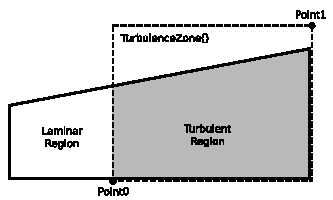
\includegraphics[width=10cm]{./chap1-introduction/figs/turbulence-zone.pdf}
 \end{center}
 \caption{Specification for a \texttt{TurbulenceZone()}}
 \label{turbulence-zone}
\end{figure}
%
In the laminar regions in Eilmer3, the turbulence source terms are not 
computed and the effective turbulence viscosity is set to zero. The use of 
\texttt{TurbulenceZone()} is similar to that of the other special zones 
discussed in the Eilmer3 user guide.


%------------------------------------------------------------------
\subsection{Recommended guidelines for use of $k$-$\omega$ model in Eilmer3}
\label{section-intro-recommended-guidelines}
%
Guidelines with regards to the setting up of grids and specification of
freestream turbulence properties for turbulent CFD simulations are rather
scattered in literature, and are hence not easily accessible. As such,
the authors have gathered in this section several guidelines from a review
of the available literature and also from experience with the usage of the
turbulence model. These guidelines are as follows.

\begin{itemize}

\item \textbf{Non-dimensionalised normal distance of first cell from the wall, $y^+$} \\
The non-dimensionalised normal distance of first cell from the wall $y^+$,
defined in Equations~\ref{eqn-yplus} - \ref{eqn-wall-shear-stress}, 
%
\begin{eqnarray}
y^+ = \frac{y \, \upsilon^{\ast} \, \rho_{wall}}{\mu_{wall}}
\label{eqn-yplus} \\
\upsilon^{\ast} = \sqrt{\frac{\tau_{wall}}{\rho_{wall}}}
\label{eqn-friction-velocity} \\
\tau_{wall} \approx \mu_{wall} \left( \frac{\partial u}{\partial y} \right) _{y=0}
\label{eqn-wall-shear-stress}
\end{eqnarray}
%
is an important value to consider when doing turbulent simulations. This 
distance has a non-trivial effect on the accuracy of surface skin friction 
and heat flux \cite{Wilcox2006}. For turbulence models that integrate through 
the viscous sublayer (that is, for models that do not use wall functions
to resolve the viscous sublayer), it is essential to have at least one cell 
within the viscous sublayer. For most cases, this corresponds to the criterion that
%
\begin{eqnarray}
y^+ < 1
\end{eqnarray}

This criterion has been recommended by many authors \cite{Wilcox2006,Versteeg2007,
Tu2008,ESI2004,AeroSoft2009,Fluent2006,Roy2003} and should be adhered to. 
The only exception for this criterion to be relaxed is in
the first few cells from the leading edge where the boundary layer has
just started developing. Although uncommon, some authors \cite{Tu2008,Fluent2006} 
noted that using a $y^+$ of up to 5 is marginally acceptable only if the first 
cell is still within the viscous sublayer (that is, if $y^+\,=\,u^+$). For 
simulations that uses wall functions to resolve the viscous sublayer, larger 
$y^+$ values (between 10 and 100) can be used \cite{Wilcox2006}. For 
shock-separated hypersonic flows, using a $y^+$ of less than 0.3 is 
recommended \cite{Wilcox2006}.

\item \textbf{Minimum number of cells within boundary layer} \\
The use of a minimum of 10 to 20 cells within the boundary layer is commonly recommended
\cite{Hirsch2007,Versteeg2007,Fluent2006}. This criterion is required to allow sufficient
resolution of the profile across the boundary layer. To capture shock separated boundary
layers, some researchers have gone to the extent of having 90 cells to resolve the boundary
layer profile \cite{Boyce2000}. As with the criterion for $y^+$, this criterion can also be
relaxed for the first few cells from the leading edge where the boundary layer has just
started developing.

\item \textbf{Maximum aspect ratio of cells} \\
Unlike the recommendations for $y^+$ and minimum number of cells required in the
boundary layer, those for maximum cell aspect ratios are not as clear. Some authors
\cite{Tu2008,Fluent2006} recommend having cell aspect ratios of less than 5 in
non-boundary-layer portions of the flow. Although these authors noted that this criterion can
be relaxed in boundary layer regions, no value for the maximum cell aspect ratio in these regions is specified.
Hirsch \cite{Hirsch1988,Hirsch2007} noted that aspect ratios larger than 100 and in the order of
1000 are not uncommon for first wall cells. Hirsh also mentioned that the use of high cell aspect
ratios is acceptable as long as near-wall cells are sufficiently orthogonal. 
It is commonly agreed that having high cell aspect ratios in CFD simulations can lead to the
degradation of computation accuracy. However, for viscous simulations in which the first cell
has to be placed extremely close to the wall in order to capture the viscous effects,
restricting cell aspect ratios to less than 5 may not be practical. From the axisymmetric
cylinder test case shown later in Section~\ref{chapter-cylinder} report, using cells with 
aspect ratios higher than 600 appear to cause the simulations to become unstable and give 
erroneous results. As this recommendation is deduced from a test case which had relatively 
simple flow, it is highly likely that a smaller aspect ratio is needed in regions with 
stronger flow gradients or flow separation. Nonetheless, the value of 600 can be used as 
an upper limit for maximum aspect ratio of near-wall cells.

\item \textbf{Freestream turbulence properties - turbulence kinetic energy, $k$ 
and specific dissipation rate, $\omega$} \\
As mentioned before, $k$ and $\omega$ can be specified as turbulence intensity
and turbulent-to-laminar viscosity ratio respectively. 
Turbulence intensity can usually be measured experimentally. Commonly used values of 
turbulence intensity range from 0.00001 to 0.1 \cite{Roy2003,Fluent2006}. The value of 
0.00001 for turbulence intensity is representative of that in free flight while the value 
of 0.1 is representative of that in wind tunnels downstream of turbulence-generating screens.
Unlike the turbulence intensity, values for turbulent-to-laminar viscosity ratio cannot
be measured easily. Commonly recommended values range from 0.00001 to 100 \cite{Roy2003,Fluent2006,
ESI2004,Tu2008}. Freestream values of $/omega$ computed from turbulence intensity and
turbulent-to-laminar viscosity ratio should also be checked that they are not larger
than 1\% of the peak value in turbulent regions, since using these values is considered
to be unrealistic \cite{Wilcox2006}.

\end{itemize}

Despite the time and computational resources required, it is recommended that 
sensitivity studies of the above mentioned parameters be performed
to ascertain the accuracy and robustness of the turbulence model.

%------------------------------------------------------------------
%\subsection{Summary of test cases}
%\label{}
%
%The first validation test case is that of a two-dimensional Mach 3.7
%flow over a flat plate. In this exercise, Eilmer3 simulation results are compared with
%the experimental results of Coles (1953) and van Driest's (1956) theoretical 
%correlation for skin friction on a flat
%plate. The sensitivity of the $k$-$\omega$ model to freestream turbulence
%properties are also examined.
%
%The second validation test case is that of a Mach 8.8 flow
%over a hollow cylinder. This test case is basically an axisymmetric
%analogy of the flat plate test case examined in Chapter~\ref{chapter-flat-plate}.
%It serves as an excellent exercise to test the axisymmetric turbulence
%terms in the $k$-$\omega$ model. The large experimental data set of surface
%pressure and heat flux provided in Mallinson et al (2000) and in Boyce \& Hillier
%(2000) is compared with predictions from Eilmer3 simulations. The sensitivity of 
%the $k$-$\omega$ model to different meshing parameters are also examined.
%
%The third validation test case is that of a Mach 2.0 flow over a
%two-dimensional backward-facing step. Experimental data from Eklund et. al. (1995)
%and McDaniel et. al. (1991) is used for this exercise.
%
%The fourth validation test case is that of experiments involving the
%turbulent mixing of supersonic coaxial jets. Conducted at NASA
%Langley Research Centre, these experiments have been adopted by
%the NATO Research and Technology Organisation Working Group 10
%(Subgroup 2) as a test case for their CFD development and validation
%activity. The reference for this test case can be found in Cutler et. al. (2006).
%
%%------------------------------------------------------------------
% SECTION OBSOLETE AS OF 16 OCTOBER 2009
% JUST FEEL THAT IT IS NOT REALLY NECESSARY IN THIS CONTEXT
%\subsection{Validation approach}
%\label{}
%
%* Discuss grid convergence, time convergence, etc.. mostly based
%on Roy and Blottner's 2003 methodology
%* Discuss why 2D cases were picked
%* State test cases in summarised table
%
%------------------------------------------------------------------
